\documentclass[a4paper,11pt,dvipdfmx]{ujarticle}
% パッケージ
\usepackage{graphicx}
\usepackage{url}
% レイアウト指定を記述したファイルの読み込み
\input{layout}

% タイトルと氏名を変更せよ.
\title{日本におけるデジタル化の状況}
\author{G58432-2025 亀井 希美}

\begin{document}

\maketitle
 %ここにタイトルが入る
 \section{デジタル競争力ランキング}

% ここから本文
国際経営開発研究所(IMD)の調査\cite{imd}によると、日本のデジタル競争力のランキングは
図\ref{fig:myfig}に示すように、調査対象の64ヶ国中、総合で28位、知識分野で25位となっている。
\begin{figure}[htbp]
    \centering
    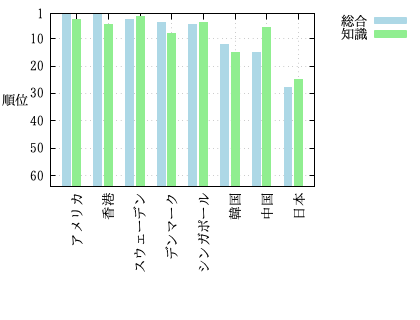
\includegraphics{fig31.png}
    \caption{デジタル競争力ランキング}\label{fig:myfig}
\end{figure}

\section{ブロードバンドの整備状況}
% を使う
OECDによるブロードバンド回線の普及に関する調査\cite{oecd}によると、表\ref{tbl:myTbl}に示すように,
日本における 100人あたりのモバイルブロードバンドの加入者数は(190.5\%)で,第一位になっている。
2位はエストニアで、3位米国と続く。

\begin{table}[htbp]
    \centering
     \caption{モバイルブロードバンドの加入数(100人あたり)}\label{tbl:myTbl}
     \begin{tabular}{|c|c|c|}
      \hline
      順位&国名&加入数\\
      \hline
     1位&日本&190.5\\
     \hline
     2位&エストニア&179.9\\
     \hline
     3位&米国&169.0\\
     \hline
     4位&フィンランド&157.0\\
     \hline
     5位&デンマーク&141.7\\
     \hline
     6位&ラトビア&141.6\\
     \hline
     7位&イスラエル&139.9\\
     \hline
     8位&オランダ&133.7\\
     \hline
     9位&ポーランド&131.3\\
     \hline
     10位&スウェーデン&127.2\\
     \hline
    \end{tabular}  
\end{table}  


% 本文(1)
%  参考文献の参照: \cite{}
%  図番号の参照: \ref{}
% を使う
% 文献データベースのキーワードは oecd と imd
% になっている.

% 図の挿入
% \includegraphics{}
% を
% \begin{figure}[htbp]
% \end{figure}
% で囲み
% \caption{}
% で図のタイトルを入れる.
% \label{}
% を使って図番号が参照できるようにする
% また,
% \centering
% で図が中央に来るようにする

% ーーー
% 節見出し(2)

% 本文(2)

% 表の挿入
% \begin{tabular}
% \end{tabular}    
% による表の記述を 
% \begin{table}[htbp]
% \begin{table}[htbp]
% で囲み
% \caption{}
% で表のタイトルを入れる.
% \label{}
% を使って表番号が参照できるようにする
% また,
% \centering
% で表が中央に来るようにする

% ーーー
% 見出し(3)
\section{考察}


% 考察
\begin{itemize}
    \item デジタル競争力ランキングは他の国と比べて低い
    \item 反対にモバイルブロードバンドの加入数は多い
    \item したがって、上位の国と比べてデジタル化が進んでいない
\end{itemize}
% \end{itemize}
\bibliographystyle{junsrt}
\bibliography{exercise.bib}

\end{document}